% Options for packages loaded elsewhere
\PassOptionsToPackage{unicode}{hyperref}
\PassOptionsToPackage{hyphens}{url}
%
\documentclass[
]{article}
\usepackage{amsmath,amssymb}
\usepackage{setspace}
\usepackage{iftex}
\ifPDFTeX
  \usepackage[T1]{fontenc}
  \usepackage[utf8]{inputenc}
  \usepackage{textcomp} % provide euro and other symbols
\else % if luatex or xetex
  \usepackage{unicode-math} % this also loads fontspec
  \defaultfontfeatures{Scale=MatchLowercase}
  \defaultfontfeatures[\rmfamily]{Ligatures=TeX,Scale=1}
\fi
\usepackage[]{libertine}
\ifPDFTeX\else
  % xetex/luatex font selection
\fi
% Use upquote if available, for straight quotes in verbatim environments
\IfFileExists{upquote.sty}{\usepackage{upquote}}{}
\IfFileExists{microtype.sty}{% use microtype if available
  \usepackage[]{microtype}
  \UseMicrotypeSet[protrusion]{basicmath} % disable protrusion for tt fonts
}{}
\makeatletter
\@ifundefined{KOMAClassName}{% if non-KOMA class
  \IfFileExists{parskip.sty}{%
    \usepackage{parskip}
  }{% else
    \setlength{\parindent}{0pt}
    \setlength{\parskip}{6pt plus 2pt minus 1pt}}
}{% if KOMA class
  \KOMAoptions{parskip=half}}
\makeatother
\usepackage{xcolor}
\usepackage[margin=1in]{geometry}
\usepackage{color}
\usepackage{fancyvrb}
\newcommand{\VerbBar}{|}
\newcommand{\VERB}{\Verb[commandchars=\\\{\}]}
\DefineVerbatimEnvironment{Highlighting}{Verbatim}{commandchars=\\\{\}}
% Add ',fontsize=\small' for more characters per line
\usepackage{framed}
\definecolor{shadecolor}{RGB}{248,248,248}
\newenvironment{Shaded}{\begin{snugshade}}{\end{snugshade}}
\newcommand{\AlertTok}[1]{\textcolor[rgb]{0.94,0.16,0.16}{#1}}
\newcommand{\AnnotationTok}[1]{\textcolor[rgb]{0.56,0.35,0.01}{\textbf{\textit{#1}}}}
\newcommand{\AttributeTok}[1]{\textcolor[rgb]{0.13,0.29,0.53}{#1}}
\newcommand{\BaseNTok}[1]{\textcolor[rgb]{0.00,0.00,0.81}{#1}}
\newcommand{\BuiltInTok}[1]{#1}
\newcommand{\CharTok}[1]{\textcolor[rgb]{0.31,0.60,0.02}{#1}}
\newcommand{\CommentTok}[1]{\textcolor[rgb]{0.56,0.35,0.01}{\textit{#1}}}
\newcommand{\CommentVarTok}[1]{\textcolor[rgb]{0.56,0.35,0.01}{\textbf{\textit{#1}}}}
\newcommand{\ConstantTok}[1]{\textcolor[rgb]{0.56,0.35,0.01}{#1}}
\newcommand{\ControlFlowTok}[1]{\textcolor[rgb]{0.13,0.29,0.53}{\textbf{#1}}}
\newcommand{\DataTypeTok}[1]{\textcolor[rgb]{0.13,0.29,0.53}{#1}}
\newcommand{\DecValTok}[1]{\textcolor[rgb]{0.00,0.00,0.81}{#1}}
\newcommand{\DocumentationTok}[1]{\textcolor[rgb]{0.56,0.35,0.01}{\textbf{\textit{#1}}}}
\newcommand{\ErrorTok}[1]{\textcolor[rgb]{0.64,0.00,0.00}{\textbf{#1}}}
\newcommand{\ExtensionTok}[1]{#1}
\newcommand{\FloatTok}[1]{\textcolor[rgb]{0.00,0.00,0.81}{#1}}
\newcommand{\FunctionTok}[1]{\textcolor[rgb]{0.13,0.29,0.53}{\textbf{#1}}}
\newcommand{\ImportTok}[1]{#1}
\newcommand{\InformationTok}[1]{\textcolor[rgb]{0.56,0.35,0.01}{\textbf{\textit{#1}}}}
\newcommand{\KeywordTok}[1]{\textcolor[rgb]{0.13,0.29,0.53}{\textbf{#1}}}
\newcommand{\NormalTok}[1]{#1}
\newcommand{\OperatorTok}[1]{\textcolor[rgb]{0.81,0.36,0.00}{\textbf{#1}}}
\newcommand{\OtherTok}[1]{\textcolor[rgb]{0.56,0.35,0.01}{#1}}
\newcommand{\PreprocessorTok}[1]{\textcolor[rgb]{0.56,0.35,0.01}{\textit{#1}}}
\newcommand{\RegionMarkerTok}[1]{#1}
\newcommand{\SpecialCharTok}[1]{\textcolor[rgb]{0.81,0.36,0.00}{\textbf{#1}}}
\newcommand{\SpecialStringTok}[1]{\textcolor[rgb]{0.31,0.60,0.02}{#1}}
\newcommand{\StringTok}[1]{\textcolor[rgb]{0.31,0.60,0.02}{#1}}
\newcommand{\VariableTok}[1]{\textcolor[rgb]{0.00,0.00,0.00}{#1}}
\newcommand{\VerbatimStringTok}[1]{\textcolor[rgb]{0.31,0.60,0.02}{#1}}
\newcommand{\WarningTok}[1]{\textcolor[rgb]{0.56,0.35,0.01}{\textbf{\textit{#1}}}}
\usepackage{graphicx}
\makeatletter
\def\maxwidth{\ifdim\Gin@nat@width>\linewidth\linewidth\else\Gin@nat@width\fi}
\def\maxheight{\ifdim\Gin@nat@height>\textheight\textheight\else\Gin@nat@height\fi}
\makeatother
% Scale images if necessary, so that they will not overflow the page
% margins by default, and it is still possible to overwrite the defaults
% using explicit options in \includegraphics[width, height, ...]{}
\setkeys{Gin}{width=\maxwidth,height=\maxheight,keepaspectratio}
% Set default figure placement to htbp
\makeatletter
\def\fps@figure{htbp}
\makeatother
\setlength{\emergencystretch}{3em} % prevent overfull lines
\providecommand{\tightlist}{%
  \setlength{\itemsep}{0pt}\setlength{\parskip}{0pt}}
\setcounter{secnumdepth}{5}
\usepackage{setspace}
\setstretch{1.2}
\usepackage{float}
\floatplacement{figure}{H}
\ifLuaTeX
  \usepackage{selnolig}  % disable illegal ligatures
\fi
\usepackage{bookmark}
\IfFileExists{xurl.sty}{\usepackage{xurl}}{} % add URL line breaks if available
\urlstyle{same}
\hypersetup{
  pdftitle={Data Visualization in R},
  pdfauthor={Eloi Vilella},
  hidelinks,
  pdfcreator={LaTeX via pandoc}}

\title{\textbf{Data Visualization in R}}
\author{Eloi Vilella}
\date{20 September 2024}

\begin{document}
\maketitle

{
\setcounter{tocdepth}{2}
\tableofcontents
}
\setstretch{1.2}
\subsection{Introduction}\label{introduction}

The following examples will walk you through the basic components of the
\texttt{ggplot2} grammar. The examples use data from the
\texttt{datasets} package, which is already loaded by default in the
\texttt{R} session, as well as some data sets loaded with
\texttt{ggplot2} package. \texttt{ggplot2} requires data to be stored in
data frames and in a \textbf{long format} (one observation per row and
one variable per column). In some cases, the \textbf{wide format} is
also used. For example, \texttt{mtcars} dataset is in \textbf{wide
format}:

\begin{Shaded}
\begin{Highlighting}[]
\FunctionTok{head}\NormalTok{(mtcars)}
\end{Highlighting}
\end{Shaded}

\begin{verbatim}
##                    mpg cyl disp  hp drat    wt  qsec vs am gear carb
## Mazda RX4         21.0   6  160 110 3.90 2.620 16.46  0  1    4    4
## Mazda RX4 Wag     21.0   6  160 110 3.90 2.875 17.02  0  1    4    4
## Datsun 710        22.8   4  108  93 3.85 2.320 18.61  1  1    4    1
## Hornet 4 Drive    21.4   6  258 110 3.08 3.215 19.44  1  0    3    1
## Hornet Sportabout 18.7   8  360 175 3.15 3.440 17.02  0  0    3    2
## Valiant           18.1   6  225 105 2.76 3.460 20.22  1  0    3    1
\end{verbatim}

where each column represents a different variable.

\subsubsection{Organization of the
practical}\label{organization-of-the-practical}

You will see different icons through the document, the meaning of which
is:

 : additional or useful information  : a worked example  : a practical
exercise  : a space to answer the exercise  : a hint to solve an
exercise  : a more challenging exercise

\texttt{ggplot2} is a data visualization package for the statistical
programming language R. Created by Hadley Wickham in 2005,
\texttt{ggplot2} is an implementation of Leland Wilkinson's Grammar of
Graphics --- a general scheme for data visualization which breaks up
graphs into semantic components such as scales and layers. We will
further learn about \texttt{ggplot2} in our next theoretical session.

\begin{center}\rule{0.5\linewidth}{0.5pt}\end{center}

\subsection{\texorpdfstring{\textbf{ Example 1} \textbar{} Creating a
scatter
plot}{ Example 1 \textbar{} Creating a scatter plot}}\label{example-1-creating-a-scatter-plot}

\subsubsection{\texorpdfstring{\textbf{1a} \textbar{} Basic scatter
plot}{1a \textbar{} Basic scatter plot}}\label{a-basic-scatter-plot}

For the first problem we want to represent the relationship between the
variables \texttt{wt} (weight) and \texttt{mpg} (miles/gallon) from the
\texttt{mtcars} data frame.

The data was extracted from the 1974 Motor Trend US magazine, and
comprises fuel consumption and 10 aspects of automobile design and
performance for 32 automobiles (1973--74 models). You can type
\texttt{?mtcars} in the \texttt{R} console to read a description of the
data.

To represent any graph in \texttt{ggplot2} we need two basic functions
that are combined with a \texttt{+} sign.

\begin{Shaded}
\begin{Highlighting}[]
\CommentTok{\# Run install.packages("ggplot2") if ggplot2 is not yet installed}
\FunctionTok{library}\NormalTok{(ggplot2)}
\FunctionTok{ggplot}\NormalTok{(}\AttributeTok{data =}\NormalTok{ mtcars, }\AttributeTok{mapping =} \FunctionTok{aes}\NormalTok{(}\AttributeTok{x =}\NormalTok{ wt, }\AttributeTok{y =}\NormalTok{ mpg)) }\SpecialCharTok{+} 
  \FunctionTok{geom\_point}\NormalTok{()}
\end{Highlighting}
\end{Shaded}

\begin{center}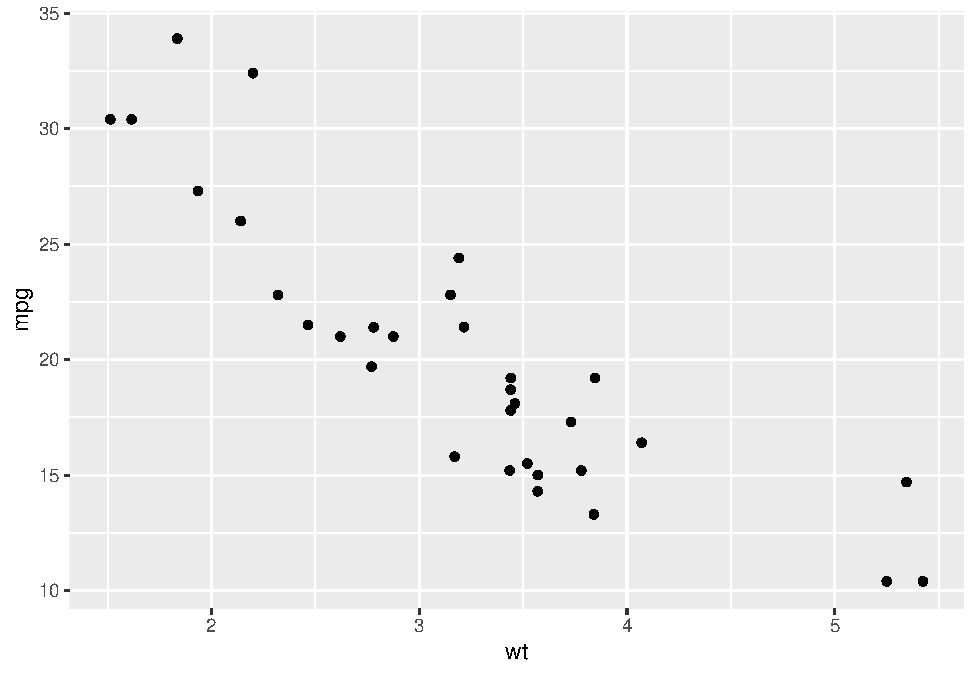
\includegraphics{P1_exercises_files/figure-latex/scatter-ggplot2-1} \end{center}

The variables that we want to represent are wrapped within an
\texttt{aes()} function, that specifies the \textbf{\emph{mapping}}
between the variables and the \textbf{\emph{aesthetic attributes}} (in
this case we map them to spatial positions, \texttt{x} and \texttt{y}).
We call the variables directly by their names, because we also pass the
entire data frame to the call with the data argument, so \texttt{ggplot}
knows were to get them from. Finally, we need to add the
\textbf{\emph{geometric object}} we want to represent. In this case,
points.

\subsubsection{\texorpdfstring{\textbf{1b} \textbar{} Represent extra
variables}{1b \textbar{} Represent extra variables}}\label{b-represent-extra-variables}

Another variable in the data indicates the number of cylinders of the
car engines (\texttt{cyl}). There are cars with 4, 6 or 8 cylinders.

\begin{Shaded}
\begin{Highlighting}[]
\FunctionTok{table}\NormalTok{(mtcars}\SpecialCharTok{$}\NormalTok{cyl)}
\end{Highlighting}
\end{Shaded}

\begin{verbatim}
## 
##  4  6  8 
## 11  7 14
\end{verbatim}

Let's say we want to represent the different types of cylinders in
different colours. In this case we want to use \texttt{cyl} as a
categorical variable, distinguishing groups rather than indicating a
value in a continuous scale. For that, we need to change its class
before giving it to \texttt{ggplot} using the \texttt{factor()}
function.

\begin{Shaded}
\begin{Highlighting}[]
\CommentTok{\# First we check the class of cyl}
\FunctionTok{class}\NormalTok{(mtcars}\SpecialCharTok{$}\NormalTok{cyl)}
\end{Highlighting}
\end{Shaded}

\begin{verbatim}
## [1] "numeric"
\end{verbatim}

\begin{Shaded}
\begin{Highlighting}[]
\CommentTok{\# Because it is numeric, let\textquotesingle{}s make cyl a factor so that we represent it as a categorical variable.}
\CommentTok{\# We create a new variable in the dataframe, cyl\_f, that is cyl converted to factor}
\NormalTok{mtcars}\SpecialCharTok{$}\NormalTok{cyl\_f }\OtherTok{\textless{}{-}} \FunctionTok{factor}\NormalTok{(mtcars}\SpecialCharTok{$}\NormalTok{cyl)}

\FunctionTok{ggplot}\NormalTok{(}\AttributeTok{data =}\NormalTok{ mtcars, }\AttributeTok{mapping =} \FunctionTok{aes}\NormalTok{(}\AttributeTok{x =}\NormalTok{ wt, }\AttributeTok{y =}\NormalTok{ mpg, }\AttributeTok{colour =}\NormalTok{ cyl\_f)) }\SpecialCharTok{+} 
  \FunctionTok{geom\_point}\NormalTok{()}
\end{Highlighting}
\end{Shaded}

\begin{center}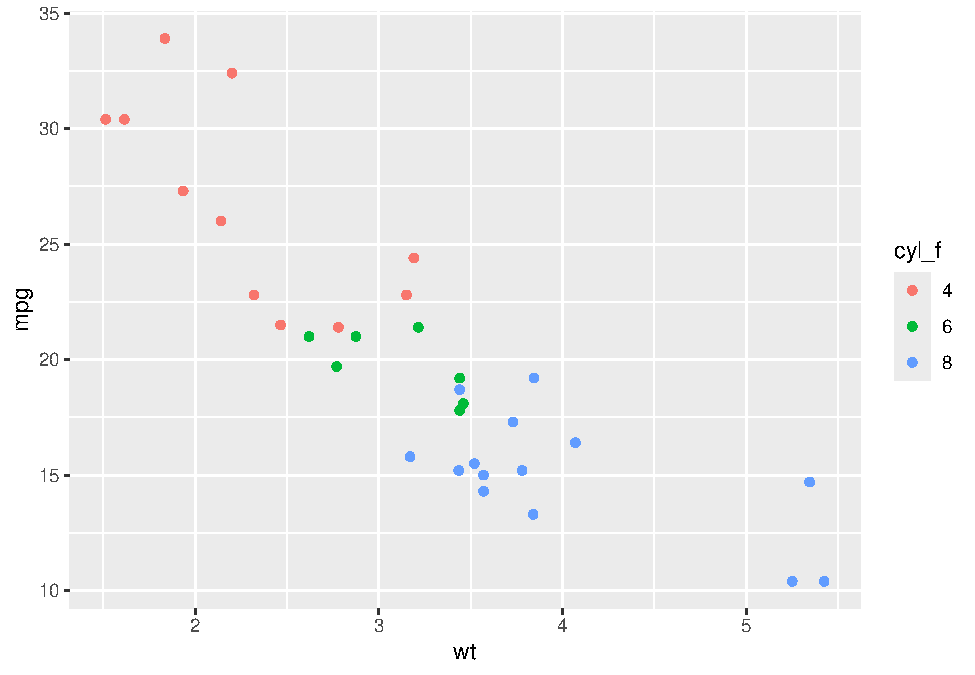
\includegraphics{P1_exercises_files/figure-latex/groups-ggplot2-1} \end{center}

Note that \texttt{ggplot} adds a \textbf{legend} by default for all the
variables that have been mapped to some aesthetic attribute. This way we
can read all the variables without extra effort.

\subsubsection{\texorpdfstring{ Exercise}{ Exercise}}\label{exercise}

Try mapping \texttt{cyl\_f} to another aesthetic attribute instead of
\texttt{colour}, such as \texttt{shape} or \texttt{size}.

\begin{Shaded}
\begin{Highlighting}[]
\CommentTok{\# Shape}
\FunctionTok{ggplot}\NormalTok{(}\AttributeTok{data =}\NormalTok{ mtcars, }\AttributeTok{mapping =} \FunctionTok{aes}\NormalTok{(}\AttributeTok{x =}\NormalTok{ wt, }\AttributeTok{y =}\NormalTok{ mpg, }\AttributeTok{shape =}\NormalTok{ cyl\_f)) }\SpecialCharTok{+} 
  \FunctionTok{geom\_point}\NormalTok{()}
\end{Highlighting}
\end{Shaded}

\begin{center}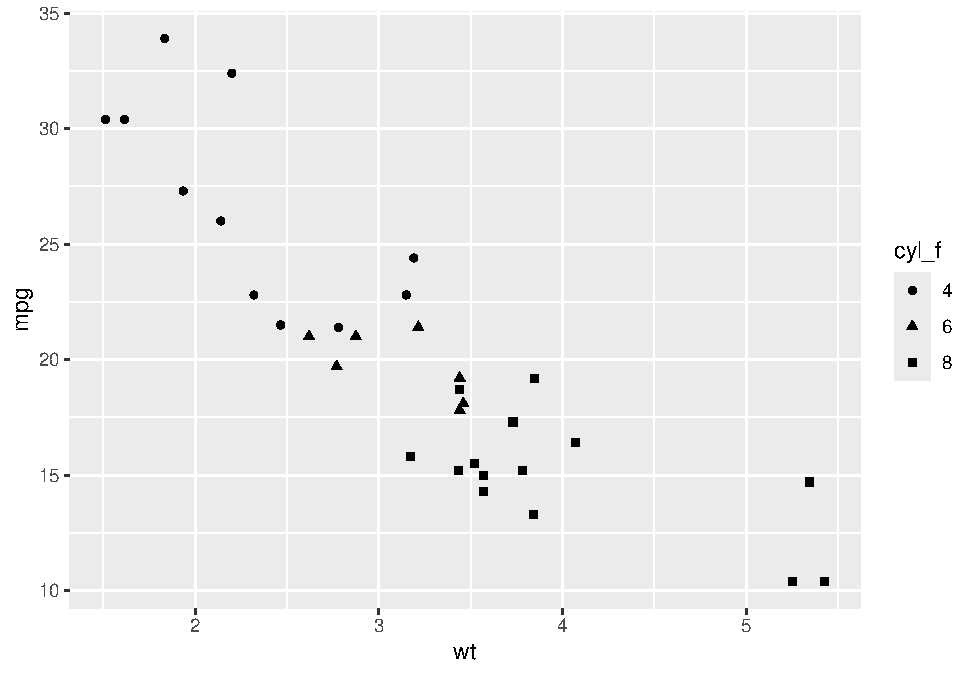
\includegraphics{P1_exercises_files/figure-latex/answer1.1-1} \end{center}

\begin{Shaded}
\begin{Highlighting}[]
\CommentTok{\# Size}
\FunctionTok{ggplot}\NormalTok{(}\AttributeTok{data =}\NormalTok{ mtcars, }\AttributeTok{mapping =} \FunctionTok{aes}\NormalTok{(}\AttributeTok{x =}\NormalTok{ wt, }\AttributeTok{y =}\NormalTok{ mpg, }\AttributeTok{size =}\NormalTok{ cyl\_f)) }\SpecialCharTok{+} 
  \FunctionTok{geom\_point}\NormalTok{()}
\end{Highlighting}
\end{Shaded}

\begin{verbatim}
## Warning: Using size for a discrete variable is not advised.
\end{verbatim}

\begin{center}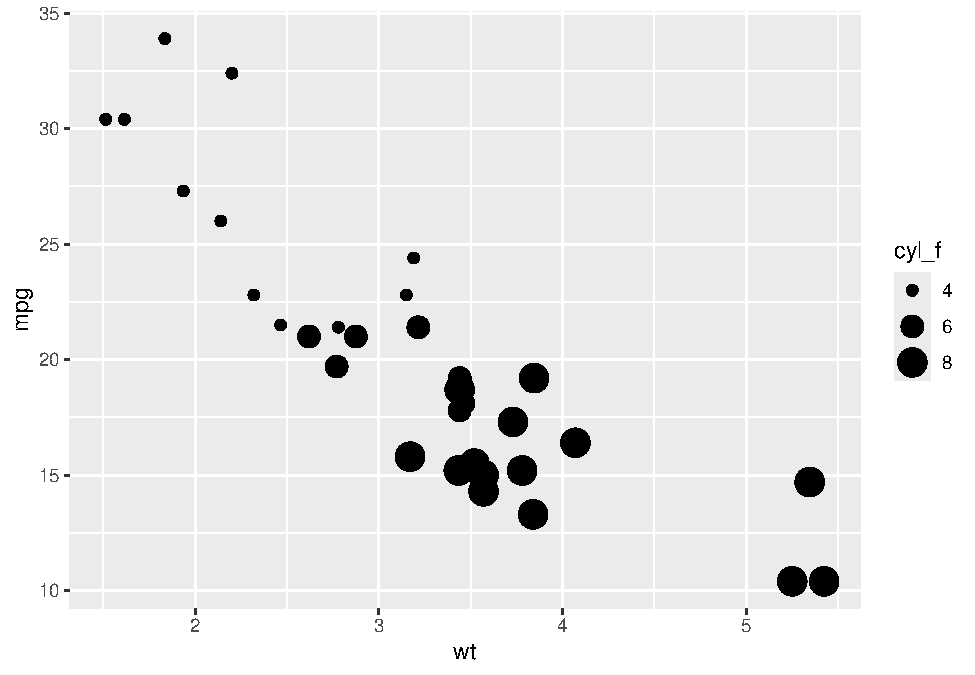
\includegraphics{P1_exercises_files/figure-latex/answer1.1-2} \end{center}

\subparagraph{  Answer:}\label{answer}

 

What happens if you map a continuous variable such as \texttt{qsec},
instead of \texttt{cyl}, to \texttt{colour}? And to \texttt{shape}?

\begin{Shaded}
\begin{Highlighting}[]
\CommentTok{\#Instead of categorical colours, it appears a gradient of 2 shades of blue which encompasses the whole continous range}
\FunctionTok{ggplot}\NormalTok{(}\AttributeTok{data =}\NormalTok{ mtcars, }\AttributeTok{mapping =} \FunctionTok{aes}\NormalTok{(}\AttributeTok{x =}\NormalTok{ wt, }\AttributeTok{y =}\NormalTok{ mpg, }\AttributeTok{colour =}\NormalTok{ qsec)) }\SpecialCharTok{+} 
  \FunctionTok{geom\_point}\NormalTok{()}
\end{Highlighting}
\end{Shaded}

\begin{center}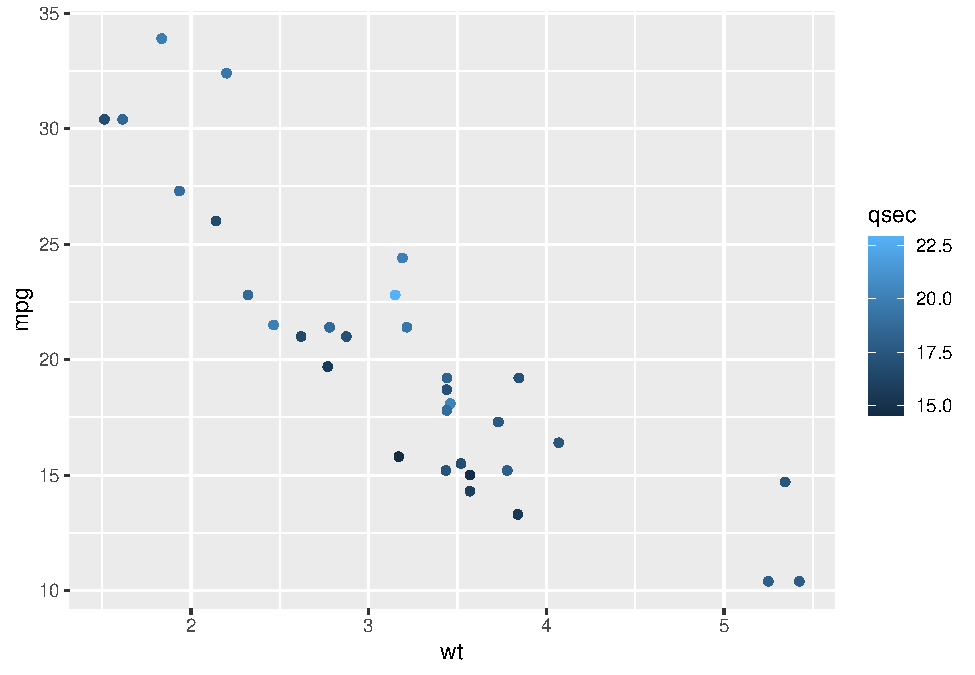
\includegraphics{P1_exercises_files/figure-latex/answer1.2-1} \end{center}

\begin{Shaded}
\begin{Highlighting}[]
\CommentTok{\# To shape is not possible due to the continous nature of our variable}
\end{Highlighting}
\end{Shaded}

\subparagraph{  Answer:}\label{answer-1}

 

\begin{center}\rule{0.5\linewidth}{0.5pt}\end{center}

\subsection{\texorpdfstring{ \textbf{Example 2} \textbar{} Creating a
bar
plot}{ Example 2 \textbar{} Creating a bar plot}}\label{example-2-creating-a-bar-plot}

\subsubsection{\texorpdfstring{\textbf{2a} \textbar{} Basic bar
plot}{2a \textbar{} Basic bar plot}}\label{a-basic-bar-plot}

We now want to summarise our data in a simple bar plot representing the
number of cars in each cylinder category. However, the number of cars
with 4 cylinders is not a piece of information present in the data set,
for example. To know the number it is necessary to count the rows where
\texttt{cyl\ =\ 4}.

\texttt{ggplot2} is capable to do simple summary operations with the
input variables, refered as \textbf{\textbf{statistical
tranformations}}. One of them is to count the occurrences of each value
in a variable. And \texttt{geom\_bar} function happen to use the
\texttt{count} statistical transformation by default on the variable
mapped to the \texttt{x} axis.

\begin{Shaded}
\begin{Highlighting}[]
\FunctionTok{ggplot}\NormalTok{(}\AttributeTok{data =}\NormalTok{ mtcars, }\AttributeTok{mapping =} \FunctionTok{aes}\NormalTok{(}\AttributeTok{x =}\NormalTok{ cyl)) }\SpecialCharTok{+}
  \FunctionTok{geom\_bar}\NormalTok{()}
\end{Highlighting}
\end{Shaded}

\begin{center}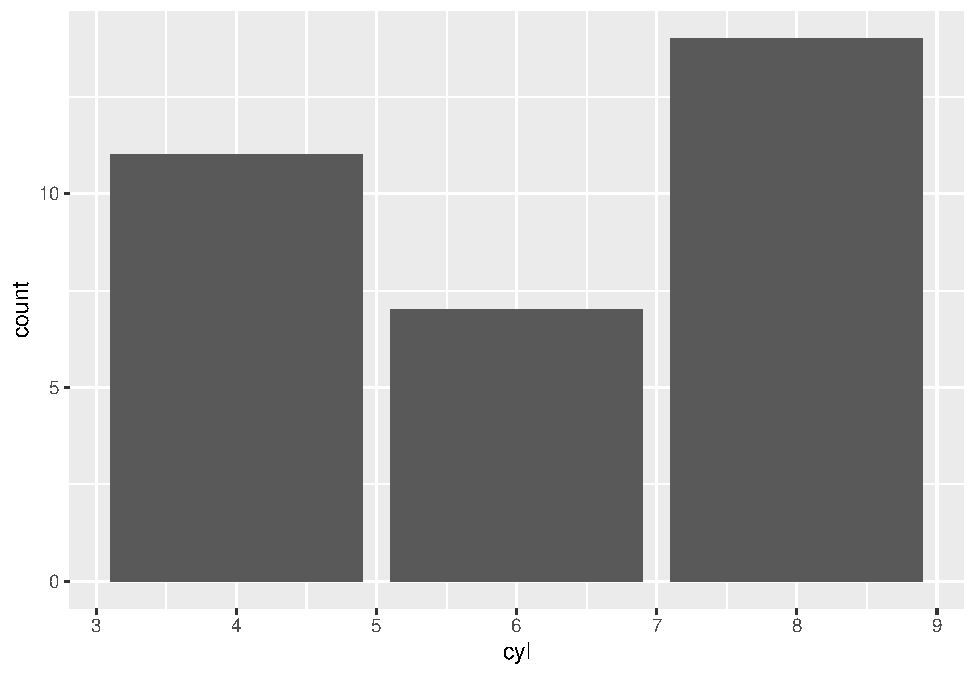
\includegraphics{P1_exercises_files/figure-latex/barplot-ggplot2-1} \end{center}

\begin{Shaded}
\begin{Highlighting}[]
\CommentTok{\# \# The same as}
 \FunctionTok{ggplot}\NormalTok{(}\AttributeTok{data =}\NormalTok{ mtcars, }\AttributeTok{mapping =} \FunctionTok{aes}\NormalTok{(}\AttributeTok{x =}\NormalTok{ cyl)) }\SpecialCharTok{+}
   \FunctionTok{geom\_bar}\NormalTok{(}\AttributeTok{stat =} \StringTok{"count"}\NormalTok{)}
\end{Highlighting}
\end{Shaded}

\begin{center}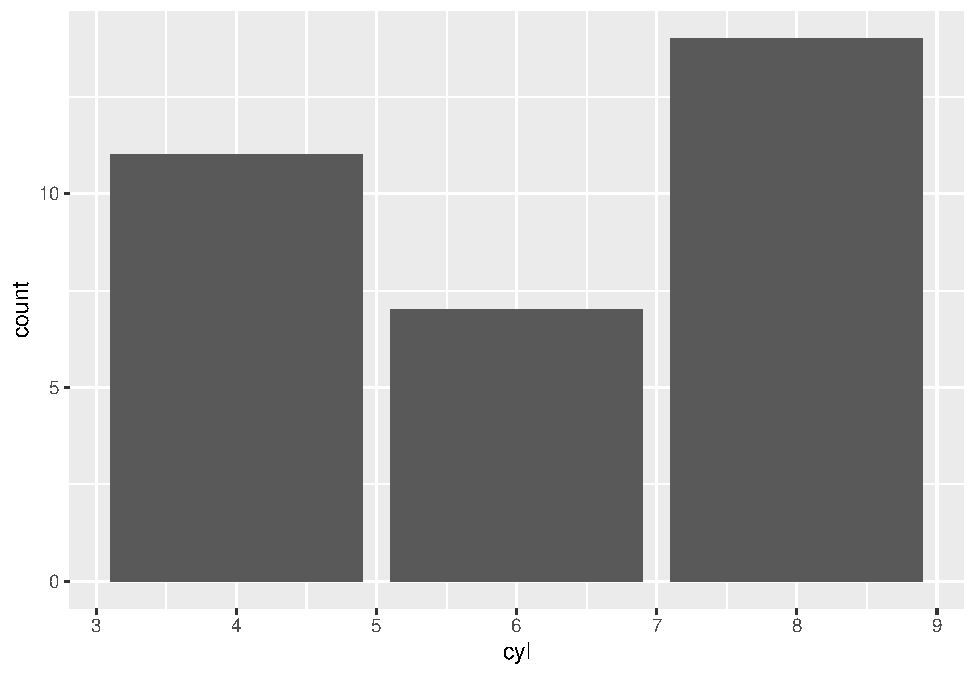
\includegraphics{P1_exercises_files/figure-latex/barplot-ggplot2-2} \end{center}

If we had a precomputed data frame with \texttt{cyl} and
\texttt{number\_of\_cars} instead, we could pass
\texttt{number\_of\_cars} variable to \texttt{geom\_col} function, that
by default takes the variables mapped to \texttt{x} and \texttt{y}
without transformation.

\begin{Shaded}
\begin{Highlighting}[]
\CommentTok{\# Let\textquotesingle{}s create the data frame}
\NormalTok{counts\_by\_cyl\_data\_frame }\OtherTok{\textless{}{-}} \FunctionTok{as.data.frame}\NormalTok{(}\FunctionTok{table}\NormalTok{(mtcars}\SpecialCharTok{$}\NormalTok{cyl))}
\FunctionTok{names}\NormalTok{(counts\_by\_cyl\_data\_frame) }\OtherTok{\textless{}{-}} \FunctionTok{c}\NormalTok{(}\StringTok{"cyl"}\NormalTok{, }\StringTok{"number\_of\_cars"}\NormalTok{)}

\CommentTok{\#ggplot(data = counts\_by\_cyl\_data\_frame, mapping = aes(x = cyl, y = number\_of\_cars)) +}
 \CommentTok{\# geom\_col()}
\end{Highlighting}
\end{Shaded}

Alternatively, we could remove the default statistical transformation of
\texttt{geom\_bar} with \texttt{stat\ =\ "indentity"} and use the
precomputed data frame.

\begin{Shaded}
\begin{Highlighting}[]
\CommentTok{\# \# The same as}
\CommentTok{\# ggplot(data = counts\_by\_cyl\_data\_frame, mapping = aes(x = cyl, y = number\_of\_cars)) +}
\CommentTok{\#   geom\_bar(stat = "identity")}
\end{Highlighting}
\end{Shaded}

\subsubsection{\texorpdfstring{\textbf{2b} \textbar{} Groups and
position}{2b \textbar{} Groups and position}}\label{b-groups-and-position}

We have seen in the scatter plot example how to represent groups encoded
in extra variables as colours. Say we now want to show transmission type
(\texttt{am}) in the bar plot, in addition to the number of cylinders.
We can map \texttt{am} to the filling colour of the bars, \texttt{fill}.
(\texttt{colour} would change the edges of the rectangles.)

\begin{Shaded}
\begin{Highlighting}[]
\CommentTok{\# First we make am factor, and we can change the 0/1 notation for a more informative notation: automatic/manual}
\NormalTok{mtcars}\SpecialCharTok{$}\NormalTok{am\_f }\OtherTok{\textless{}{-}} \FunctionTok{factor}\NormalTok{(mtcars}\SpecialCharTok{$}\NormalTok{am, }\AttributeTok{levels =} \FunctionTok{c}\NormalTok{(}\DecValTok{0}\NormalTok{, }\DecValTok{1}\NormalTok{), }\AttributeTok{labels =} \FunctionTok{c}\NormalTok{(}\StringTok{"automatic"}\NormalTok{,}\StringTok{"manual"}\NormalTok{))}

\FunctionTok{ggplot}\NormalTok{(}\AttributeTok{data =}\NormalTok{ mtcars, }\AttributeTok{mapping =} \FunctionTok{aes}\NormalTok{(}\AttributeTok{x =}\NormalTok{ cyl, }\AttributeTok{fill =}\NormalTok{ am\_f)) }\SpecialCharTok{+}
  \FunctionTok{geom\_bar}\NormalTok{()}
\end{Highlighting}
\end{Shaded}

\begin{center}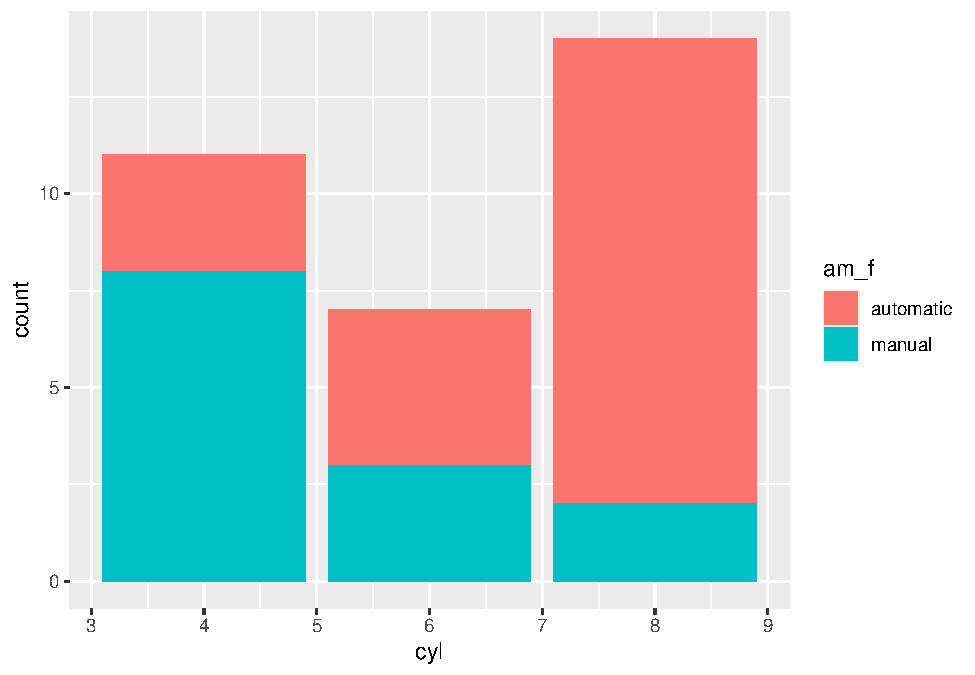
\includegraphics{P1_exercises_files/figure-latex/groups-bar-1} \end{center}

Each geometric object in \texttt{ggplot2} also has a
\textbf{\textbf{position}} argument that controls how groups are
arranged. In \texttt{geom\_bar} the default position is to stack any
groups. We can change it for a side-by-side position with
\texttt{position\ =\ "dodge"}.

\begin{Shaded}
\begin{Highlighting}[]
\FunctionTok{ggplot}\NormalTok{(}\AttributeTok{data =}\NormalTok{ mtcars, }\AttributeTok{mapping =} \FunctionTok{aes}\NormalTok{(}\AttributeTok{x =}\NormalTok{ cyl, }\AttributeTok{fill =}\NormalTok{ am\_f)) }\SpecialCharTok{+}
  \FunctionTok{geom\_bar}\NormalTok{(}\AttributeTok{position =} \StringTok{"dodge"}\NormalTok{)}
\end{Highlighting}
\end{Shaded}

\begin{center}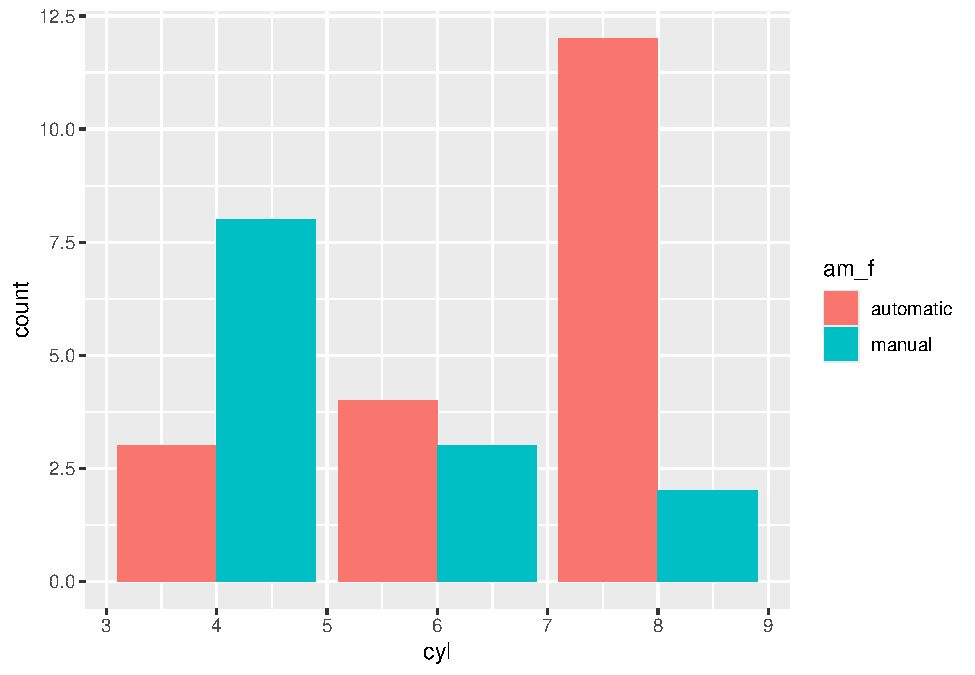
\includegraphics{P1_exercises_files/figure-latex/position-bar-ggplot2-1} \end{center}

\subsubsection{\texorpdfstring{ Exercise}{ Exercise}}\label{exercise-1}

Which is the \texttt{position} argument in the \texttt{ggplot2} bar plot
that standardises the bars to the same height? Update the plot above
with the new position adjustment.

\begin{Shaded}
\begin{Highlighting}[]
\CommentTok{\# The argument is fill}
\FunctionTok{ggplot}\NormalTok{(}\AttributeTok{data =}\NormalTok{ mtcars, }\AttributeTok{mapping =} \FunctionTok{aes}\NormalTok{(}\AttributeTok{x =}\NormalTok{ cyl, }\AttributeTok{fill =}\NormalTok{ am\_f)) }\SpecialCharTok{+}
  \FunctionTok{geom\_bar}\NormalTok{(}\AttributeTok{position =} \StringTok{"fill"}\NormalTok{)}
\end{Highlighting}
\end{Shaded}

\begin{center}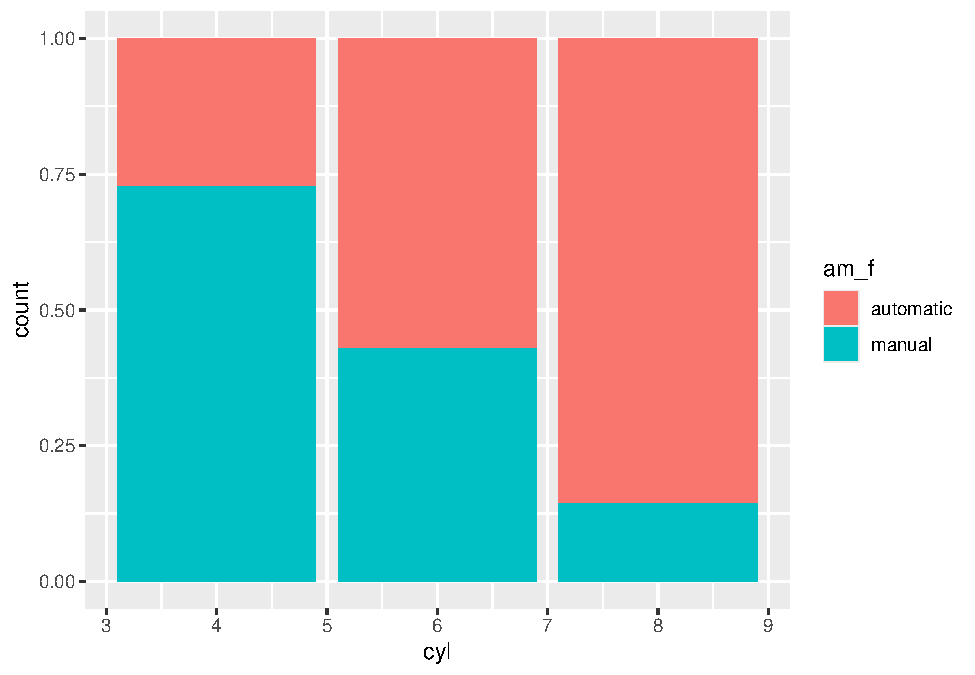
\includegraphics{P1_exercises_files/figure-latex/positions-ggplot2 answer2.1-1} \end{center}

\subparagraph{  Answer:}\label{answer-2}

 

Which position adjustment would you choose if you still wanted to
compare the total amount of cars with each cylinder category? And if you
were interested in knowing the relative abundance of each type of
transmission?

\subparagraph{  Answer:}\label{answer-3}

 

\begin{center}\rule{0.5\linewidth}{0.5pt}\end{center}

\subsection{\texorpdfstring{ \textbf{Example 3} \textbar{} Showing the
distribution of a
variable}{ Example 3 \textbar{} Showing the distribution of a variable}}\label{example-3-showing-the-distribution-of-a-variable}

\subsubsection{\texorpdfstring{\textbf{3a} \textbar{} Simple
histogram}{3a \textbar{} Simple histogram}}\label{a-simple-histogram}

Now we have a new data set called \texttt{iris} and we need to
understand the distribution of some of its continuous variables. A good
place to start is a histogram, that represents the number of
observations in different ranges as bars.

Note that histograms deal with \emph{continuous} variables while bar
plots with \emph{discrete}, but are sometimes
\href{https://www.google.com/search?q=histograms+and+bar+graphs+difference}{confused}.

The function that we need is called \texttt{geom\_histogram} and has the
statistical transformation \texttt{bin} by default. In this case,
\texttt{bin} divides the variable mapped to \texttt{x} in ranges and
counts the number of values in each bin. The number of bins is
controlled with the argument \texttt{binwidth}.

\begin{Shaded}
\begin{Highlighting}[]
\FunctionTok{ggplot}\NormalTok{(}\AttributeTok{data =}\NormalTok{ iris, }\AttributeTok{mapping =} \FunctionTok{aes}\NormalTok{(}\AttributeTok{x =}\NormalTok{ Sepal.Width)) }\SpecialCharTok{+}
  \FunctionTok{geom\_histogram}\NormalTok{(}\AttributeTok{binwidth =} \FloatTok{0.1}\NormalTok{)}
\end{Highlighting}
\end{Shaded}

\begin{center}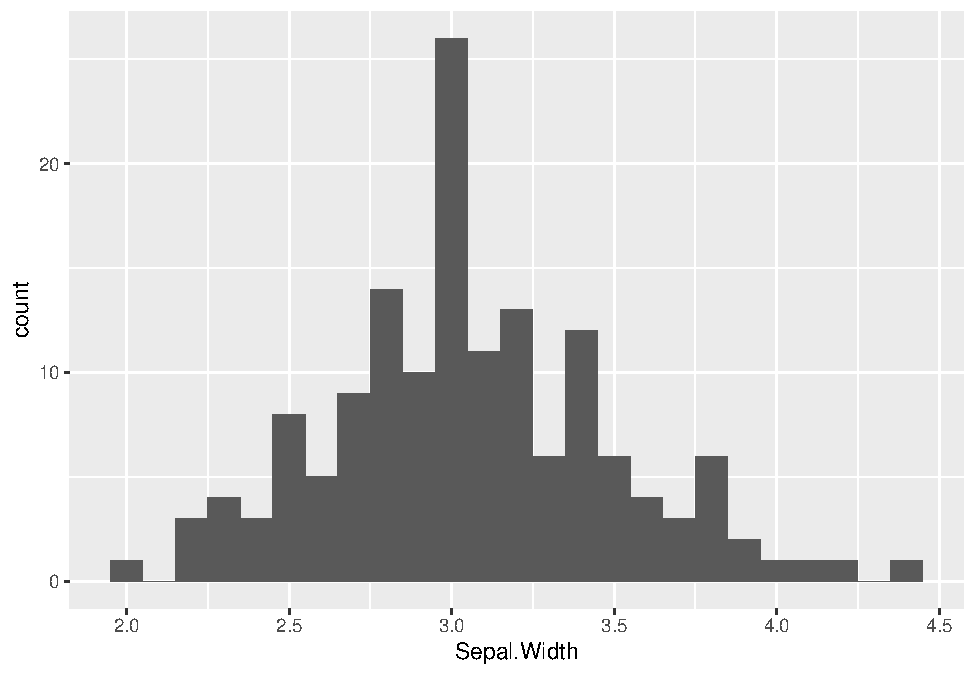
\includegraphics{P1_exercises_files/figure-latex/histogram-1} \end{center}

\subsubsection{\texorpdfstring{\textbf{3b} \textbar{} Multiple
histograms}{3b \textbar{} Multiple histograms}}\label{b-multiple-histograms}

\texttt{iris} data contains information about three species of
\href{https://en.wikipedia.org/wiki/Iris_(plant)}{iris}: \emph{setosa},
\emph{versicolor} and \emph{virginica}. To see the distribution of the
different species we can try to map the species to the filling colour.
That's easy with \texttt{ggplot2}!

\begin{Shaded}
\begin{Highlighting}[]
\FunctionTok{ggplot}\NormalTok{(}\AttributeTok{data =}\NormalTok{ iris, }\AttributeTok{mapping =} \FunctionTok{aes}\NormalTok{(}\AttributeTok{x =}\NormalTok{ Sepal.Width, }\AttributeTok{fill =}\NormalTok{ Species)) }\SpecialCharTok{+}
  \FunctionTok{geom\_histogram}\NormalTok{(}\AttributeTok{binwidth =} \FloatTok{0.1}\NormalTok{) }
\end{Highlighting}
\end{Shaded}

\begin{center}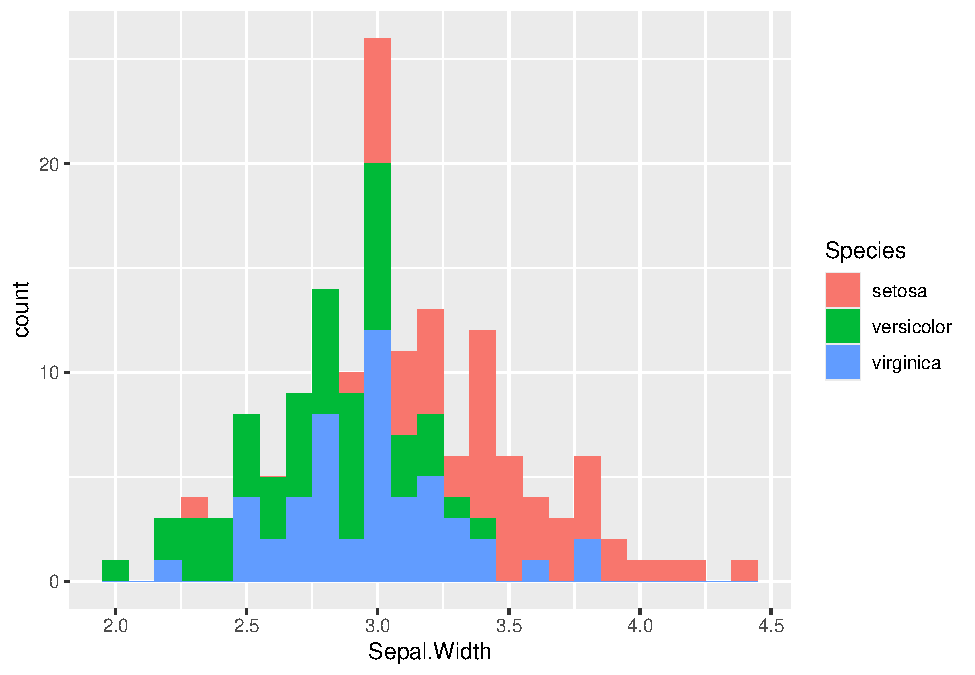
\includegraphics{P1_exercises_files/figure-latex/histogram-fill-1} \end{center}

Stacked histograms are difficult to interpret and three separated
subplots could actually work better. \texttt{ggplot2} provides a simple
way of creating small multiples or \textbf{facets} with the functions
\texttt{facet\_grid} and \texttt{facet\_wrap}.

\begin{Shaded}
\begin{Highlighting}[]
\FunctionTok{ggplot}\NormalTok{(}\AttributeTok{data =}\NormalTok{ iris, }\AttributeTok{mapping =} \FunctionTok{aes}\NormalTok{(}\AttributeTok{x =}\NormalTok{ Sepal.Width, }\AttributeTok{fill =}\NormalTok{ Species)) }\SpecialCharTok{+}
  \FunctionTok{geom\_histogram}\NormalTok{(}\AttributeTok{binwidth =} \FloatTok{0.1}\NormalTok{) }\SpecialCharTok{+}
  \FunctionTok{facet\_grid}\NormalTok{(Species }\SpecialCharTok{\textasciitilde{}}\NormalTok{ .)}
\end{Highlighting}
\end{Shaded}

\begin{center}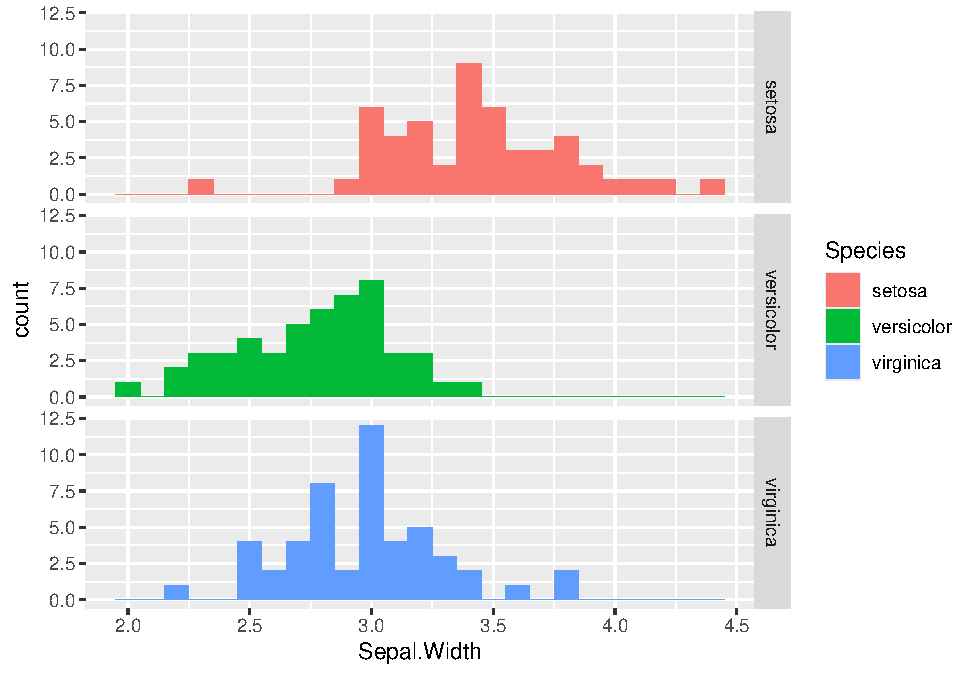
\includegraphics{P1_exercises_files/figure-latex/facets-1} \end{center}

\subsubsection{\texorpdfstring{ Exercise}{ Exercise}}\label{exercise-2}

Experiment with \texttt{facet\_grid} and \texttt{facet\_wrap}. For
testing purposes, we can create an extra categorical variable by
splitting \texttt{Petal.Length} in two groups.

\begin{Shaded}
\begin{Highlighting}[]
\NormalTok{iris}\SpecialCharTok{$}\NormalTok{Petal.Type[iris}\SpecialCharTok{$}\NormalTok{Petal.Length }\SpecialCharTok{\textgreater{}=} \DecValTok{4}\NormalTok{ ] }\OtherTok{\textless{}{-}} \StringTok{"Long"}
\NormalTok{iris}\SpecialCharTok{$}\NormalTok{Petal.Type[iris}\SpecialCharTok{$}\NormalTok{Petal.Length }\SpecialCharTok{\textless{}} \DecValTok{4}\NormalTok{ ] }\OtherTok{\textless{}{-}} \StringTok{"Short"}
\end{Highlighting}
\end{Shaded}

\subparagraph{  Answer:}\label{answer-4}

 

Which is the best subplot configuration to compare the distributions and
why?

\subparagraph{  Answer:}\label{answer-5}

 

\begin{center}\rule{0.5\linewidth}{0.5pt}\end{center}

\subsection{\texorpdfstring{ \textbf{Example 4} \textbar{} Customizing a
plot}{ Example 4 \textbar{} Customizing a plot}}\label{example-4-customizing-a-plot}

\subsubsection{\texorpdfstring{\textbf{4a} \textbar{} Modify
colours}{4a \textbar{} Modify colours}}\label{a-modify-colours}

So far we have used the default colour palettes for all our
representations. We may need to change them to make them accessible to
colourblind people, match the colour palette of our project or give
meaningful values (e.g., red for positive and blue for negative). We can
control the exact mapping of a variable to an aesthetic attribute with
the functions \texttt{scale\_*}.

\begin{Shaded}
\begin{Highlighting}[]
\FunctionTok{ggplot}\NormalTok{(}\AttributeTok{data =}\NormalTok{ iris, }\AttributeTok{mapping =} \FunctionTok{aes}\NormalTok{(}\AttributeTok{x =}\NormalTok{ Sepal.Width, }\AttributeTok{fill =}\NormalTok{ Species)) }\SpecialCharTok{+}
  \FunctionTok{geom\_histogram}\NormalTok{(}\AttributeTok{binwidth =} \FloatTok{0.1}\NormalTok{) }\SpecialCharTok{+}
  \FunctionTok{facet\_grid}\NormalTok{(Species }\SpecialCharTok{\textasciitilde{}}\NormalTok{ .) }\SpecialCharTok{+}
  \FunctionTok{scale\_fill\_manual}\NormalTok{(}\AttributeTok{values =} \FunctionTok{c}\NormalTok{(}\StringTok{"darkorange"}\NormalTok{, }\StringTok{"darkgray"}\NormalTok{, }\StringTok{"black"}\NormalTok{))}
\end{Highlighting}
\end{Shaded}

\begin{center}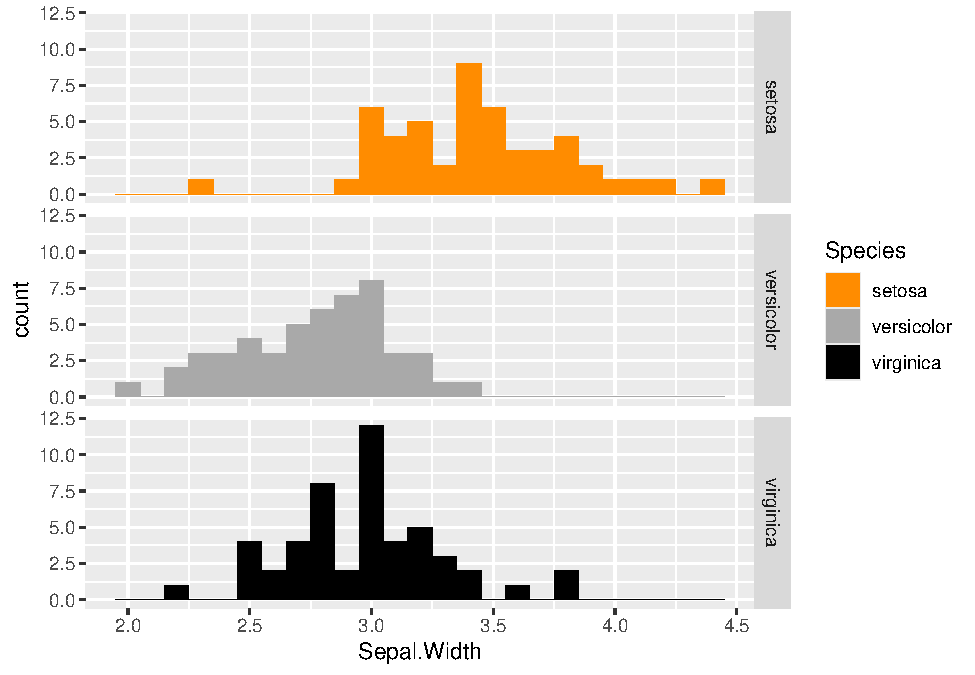
\includegraphics{P1_exercises_files/figure-latex/change-col-ggplot2-1} \end{center}

Note that scale functions update both the aesthetic mappings in the plot
and in the legend.

\subsubsection{\texorpdfstring{\textbf{4b} \textbar{} Change (or add)
axis, legend and plot
titles}{4b \textbar{} Change (or add) axis, legend and plot titles}}\label{b-change-or-add-axis-legend-and-plot-titles}

We may also need to add a title to the plot or change the axis title. In
\texttt{ggplot2} axis and legend titles can be specified with
\texttt{name} argument within a \texttt{scale\_*} function. The title is
set with \texttt{ggtitle}. You can also use the convenience function
\texttt{labs}.

\begin{Shaded}
\begin{Highlighting}[]
\CommentTok{\# We save the common part of the plot in a variable and then we can add more components with the "+" sign}
\NormalTok{p }\OtherTok{\textless{}{-}} \FunctionTok{ggplot}\NormalTok{(}\AttributeTok{data =}\NormalTok{ iris, }\AttributeTok{mapping =} \FunctionTok{aes}\NormalTok{(}\AttributeTok{x =}\NormalTok{ Sepal.Width, }\AttributeTok{fill =}\NormalTok{ Species)) }\SpecialCharTok{+}
  \FunctionTok{geom\_histogram}\NormalTok{(}\AttributeTok{binwidth =} \FloatTok{0.1}\NormalTok{) }\SpecialCharTok{+}
  \FunctionTok{facet\_grid}\NormalTok{(Species }\SpecialCharTok{\textasciitilde{}}\NormalTok{ .)}

\CommentTok{\# Option A:}
\NormalTok{p }\SpecialCharTok{+} \FunctionTok{scale\_fill\_manual}\NormalTok{(}\AttributeTok{values =} \FunctionTok{c}\NormalTok{(}\StringTok{"darkorange"}\NormalTok{, }\StringTok{"darkgray"}\NormalTok{, }\StringTok{"black"}\NormalTok{), }\AttributeTok{name =} \StringTok{"Species name"}\NormalTok{) }\SpecialCharTok{+}
  \FunctionTok{scale\_x\_continuous}\NormalTok{(}\AttributeTok{name =} \StringTok{"Sepal width"}\NormalTok{) }\SpecialCharTok{+} 
  \FunctionTok{ggtitle}\NormalTok{(}\StringTok{"Iris sepal variation"}\NormalTok{)}
\end{Highlighting}
\end{Shaded}

\begin{center}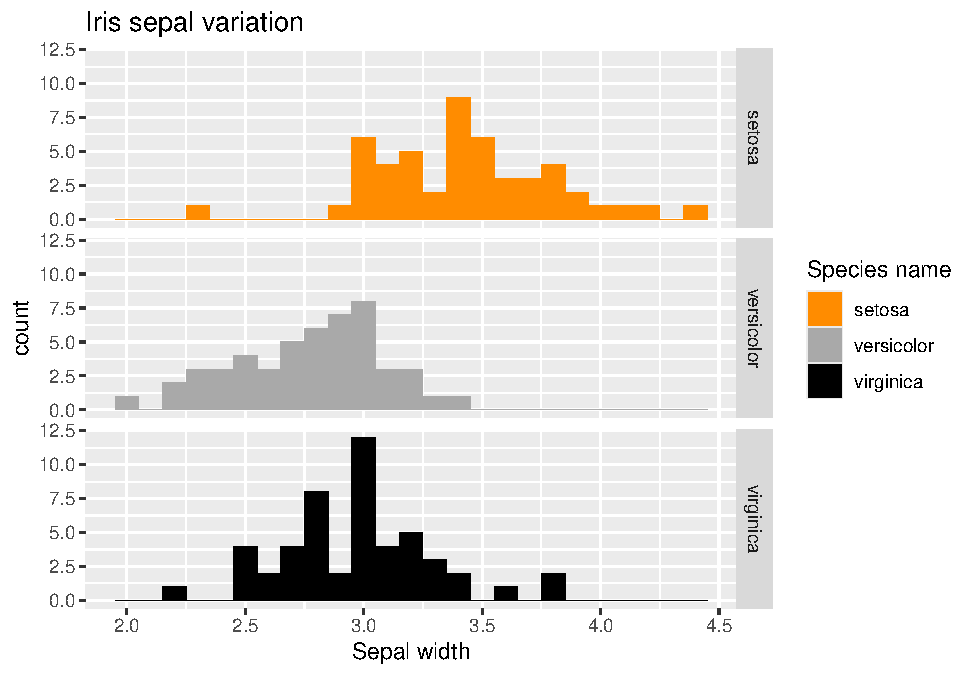
\includegraphics{P1_exercises_files/figure-latex/titles-ggplot2-1} \end{center}

\begin{Shaded}
\begin{Highlighting}[]
\CommentTok{\# Option B:}
\CommentTok{\# p + scale\_fill\_manual(values = c("darkorange", "darkgray", "black")) +}
\CommentTok{\#   labs(title = "Iris sepal variation", x = "Sepal width", fill = "Species name")}
\end{Highlighting}
\end{Shaded}

\subsubsection{\texorpdfstring{\textbf{4c} \textbar{} Change
theme}{4c \textbar{} Change theme}}\label{c-change-theme}

The appearence of \texttt{ggplot2} plots is controlled by the
\textbf{themes}. The default \texttt{ggplot2} theme has a gray
background and ``is designed to put the data forward yet make
comparisons easy''. You can change the general appearence by choosing a
different theme with \texttt{theme\_*} functions.

\begin{Shaded}
\begin{Highlighting}[]
\FunctionTok{ggplot}\NormalTok{(}\AttributeTok{data =}\NormalTok{ iris, }\AttributeTok{mapping =} \FunctionTok{aes}\NormalTok{(}\AttributeTok{x =}\NormalTok{ Sepal.Width, }\AttributeTok{y =}\NormalTok{ Sepal.Length)) }\SpecialCharTok{+}
  \FunctionTok{geom\_point}\NormalTok{() }\SpecialCharTok{+}
  \FunctionTok{theme\_classic}\NormalTok{()}
\end{Highlighting}
\end{Shaded}

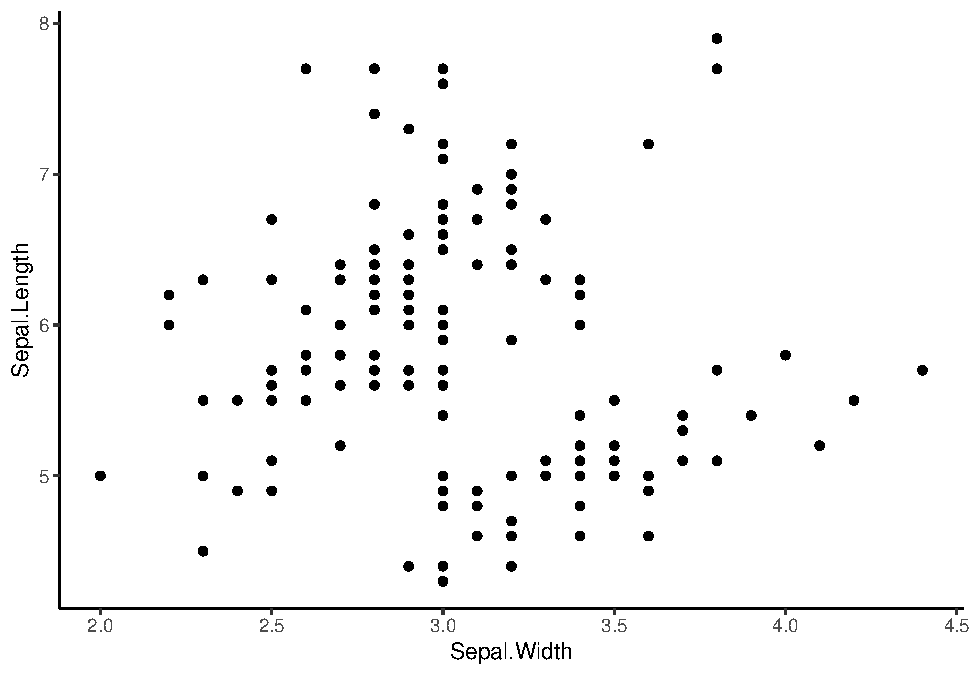
\includegraphics{P1_exercises_files/figure-latex/theme-1.pdf}

\subsubsection{\texorpdfstring{ Exercise}{ Exercise}}\label{exercise-3}

Try other \texttt{scale\_fill\_*} functions in \texttt{ggplot2} with
pre-defined palettes, such as \texttt{scale\_fill\_brewer} and
\texttt{scale\_fill\_viridis\_d}. Which palette would you use to ensure
that colourblind people can distinguish the colours?

\#Viridis palet in most colorblindcases

\subparagraph{  Answer:}\label{answer-6}

 

Try \texttt{subtitle}, \texttt{caption} and \texttt{tag} arguments from
the \texttt{labs} function. What are they for?

\subparagraph{  Answer:}\label{answer-7}

 

Which theme do you think that maximises the data-ink ratio?

\begin{Shaded}
\begin{Highlighting}[]
\FunctionTok{ggplot}\NormalTok{(}\AttributeTok{data =}\NormalTok{ iris, }\AttributeTok{mapping =} \FunctionTok{aes}\NormalTok{(}\AttributeTok{x =}\NormalTok{ Sepal.Width, }\AttributeTok{y =}\NormalTok{ Sepal.Length)) }\SpecialCharTok{+}
  \FunctionTok{geom\_point}\NormalTok{() }\SpecialCharTok{+}
  \FunctionTok{theme\_minimal}\NormalTok{() }\SpecialCharTok{+}
  \FunctionTok{labs}\NormalTok{(}\AttributeTok{x =} \StringTok{"Width"}\NormalTok{, }\AttributeTok{y =} \StringTok{"Length"}\NormalTok{)}
\end{Highlighting}
\end{Shaded}

\begin{center}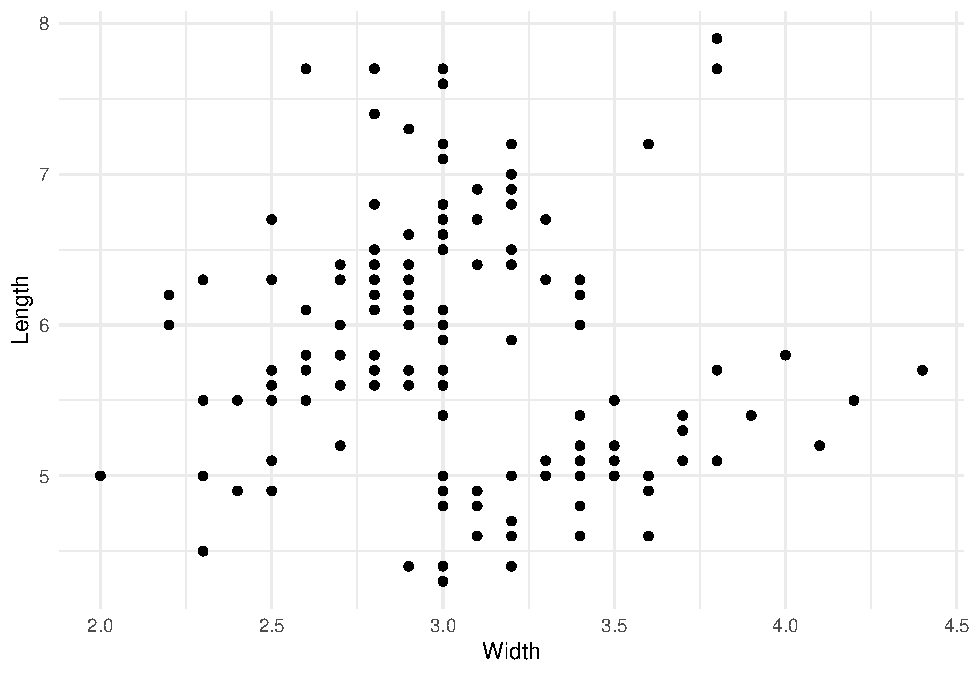
\includegraphics{P1_exercises_files/figure-latex/answer 4.1-1} \end{center}

\begin{Shaded}
\begin{Highlighting}[]
\CommentTok{\#Theme minimal}
\end{Highlighting}
\end{Shaded}

\subparagraph{  Answer:}\label{answer-8}

 

\begin{center}\rule{0.5\linewidth}{0.5pt}\end{center}

\subsection{\texorpdfstring{ Saving the
plots}{ Saving the plots}}\label{saving-the-plots}

There are three ways to save a plot to a file (from easy to difficult):

A. Export button from \texttt{RStudio} plot pane

B. \texttt{ggsave} function from \texttt{ggplot2} package

\begin{Shaded}
\begin{Highlighting}[]
\NormalTok{p }\OtherTok{\textless{}{-}} \FunctionTok{ggplot}\NormalTok{(}\AttributeTok{data =}\NormalTok{ iris, }\AttributeTok{mapping =} \FunctionTok{aes}\NormalTok{(}\AttributeTok{x =}\NormalTok{ Sepal.Width, }\AttributeTok{y =}\NormalTok{ Sepal.Length)) }\SpecialCharTok{+} \FunctionTok{geom\_point}\NormalTok{()}
\FunctionTok{ggsave}\NormalTok{(}\AttributeTok{filename =} \StringTok{"plot.png"}\NormalTok{, }\AttributeTok{plot =}\NormalTok{ p, }\AttributeTok{width =} \DecValTok{6}\NormalTok{, }\AttributeTok{height =} \DecValTok{4}\NormalTok{) }\CommentTok{\# in inches by default}
\end{Highlighting}
\end{Shaded}

C. Opening \textgreater{} Ploting \textgreater{} Closing a graphic
device

\begin{Shaded}
\begin{Highlighting}[]
\FunctionTok{png}\NormalTok{(}\AttributeTok{filename =} \StringTok{"plot.png"}\NormalTok{, }\AttributeTok{width =} \DecValTok{600}\NormalTok{, }\AttributeTok{height =} \DecValTok{400}\NormalTok{, }\AttributeTok{res =} \DecValTok{150}\NormalTok{) }\CommentTok{\# In pixels by default}
\NormalTok{p}
\FunctionTok{dev.off}\NormalTok{()}
\end{Highlighting}
\end{Shaded}

Plots can be saved using different image file formats. Option \textbf{A}
gives you the format options in a drop list, option \textbf{B} guesses
the format from the filename extension, and in option \textbf{C} the
function that is used to open the graphic device determines the format
of the output (in the example \texttt{png()}).

The main formats can be classified into:

\begin{itemize}
\tightlist
\item
  Raster/bitmat formats, where information is stored in pixels and have
  a maximum resolution.

  \begin{itemize}
  \tightlist
  \item
    \textbf{PNG}: extension .png, supports transparent background, good
    compression, doesn't lose quality
  \item
    \textbf{JPEG}: extensions .jpg and .jpeg, very good compression,
    used in personal photography but suffers from quality degradation
    with repeated modifications
  \item
    \textbf{TIFF}: extensions .tif and .tiff, preferred format for
    professional printing
  \end{itemize}
\item
  Vector formats, where information is encoded in geometric shapes that
  can be rendered at any size without losing resolution.

  \begin{itemize}
  \tightlist
  \item
    \textbf{SVG}: extension .svg, standard for vector graphics, requires
    \texttt{svglite} package
  \end{itemize}
\item
  Hybrid

  \begin{itemize}
  \tightlist
  \item
    \textbf{PDF}: can contain both vector graphics and raster images
  \end{itemize}
\end{itemize}

\subsubsection{\texorpdfstring{ Exercise}{ Exercise}}\label{exercise-4}

Save the plot \texttt{p} in a raster and a vector format with the same
size. What differences do you observe?

Note: svg devices require \texttt{svglite} R package and other system
libraries. Skip the exercise if you get an error!

\begin{Shaded}
\begin{Highlighting}[]
\CommentTok{\#install.packages("sgvlite")}

\CommentTok{\#ggsave(filename = "plot.png", plot = p, width = 6, height = 4) }
\CommentTok{\#ggsave(filename = "plot.svg", plot = p, width = 6, height = 4) }

\CommentTok{\#svg is ligther and you can do infinite zoom to its objects due to information not being stored in pixels}
\end{Highlighting}
\end{Shaded}

\subparagraph{  Answer:}\label{answer-9}

 

\begin{center}\rule{0.5\linewidth}{0.5pt}\end{center}

\subsection{\texorpdfstring{ Wrap up
exercise}{ Wrap up exercise}}\label{wrap-up-exercise}

Could you guess how to represent a line plot with \texttt{ggplot2}
syntax?

\begin{itemize}
\tightlist
\item
  Represent how \texttt{unemploy} variable changes over time
  (\texttt{date} variable) from \texttt{economics} data frame with a
  line plot using \texttt{ggplot2} syntax
\item
  Modify axis and legend names and add a title
\item
  Save the plot to a file using a raster image format
\end{itemize}

\begin{Shaded}
\begin{Highlighting}[]
\NormalTok{p }\OtherTok{\textless{}{-}} \FunctionTok{ggplot}\NormalTok{(}\AttributeTok{data =}\NormalTok{ economics, }\FunctionTok{aes}\NormalTok{(}\AttributeTok{x =}\NormalTok{ date, }\AttributeTok{y =}\NormalTok{ unemploy)) }\SpecialCharTok{+}
  \FunctionTok{geom\_line}\NormalTok{(}\AttributeTok{color =} \StringTok{"steelblue"}\NormalTok{, }\AttributeTok{size =} \DecValTok{1}\NormalTok{) }\SpecialCharTok{+}  \CommentTok{\# Enhanced line color and thickness}
  \FunctionTok{labs}\NormalTok{(}
    \AttributeTok{title =} \StringTok{"Unemployment Over Time in the US"}\NormalTok{,}
    \AttributeTok{subtitle =} \StringTok{"Monthly data from the Federal Reserve Economic Data"}\NormalTok{,}
    \AttributeTok{x =} \StringTok{"Date"}\NormalTok{,}
    \AttributeTok{y =} \StringTok{"Number of Unemployed (in thousands)"}
\NormalTok{  ) }\SpecialCharTok{+}
  \FunctionTok{theme\_minimal}\NormalTok{(}\AttributeTok{base\_size =} \DecValTok{14}\NormalTok{) }\SpecialCharTok{+}  \CommentTok{\# Cleaner theme with larger base font}
  \FunctionTok{theme}\NormalTok{(}
    \AttributeTok{plot.title =} \FunctionTok{element\_text}\NormalTok{(}\AttributeTok{face =} \StringTok{"bold"}\NormalTok{, }\AttributeTok{size =} \DecValTok{16}\NormalTok{, }\AttributeTok{hjust =} \FloatTok{0.5}\NormalTok{),  }\CommentTok{\# Centering the title}
    \AttributeTok{plot.subtitle =} \FunctionTok{element\_text}\NormalTok{(}\AttributeTok{size =} \DecValTok{12}\NormalTok{, }\AttributeTok{hjust =} \FloatTok{0.5}\NormalTok{),}
    \AttributeTok{axis.text.x =} \FunctionTok{element\_text}\NormalTok{(}\AttributeTok{angle =} \DecValTok{45}\NormalTok{, }\AttributeTok{hjust =} \DecValTok{1}\NormalTok{, }\AttributeTok{size=} \DecValTok{6}\NormalTok{)  }\CommentTok{\# Tilt x{-}axis labels for readability}
\NormalTok{  ) }\SpecialCharTok{+}
  \FunctionTok{scale\_y\_continuous}\NormalTok{(}\AttributeTok{labels =}\NormalTok{ scales}\SpecialCharTok{::}\NormalTok{comma)  }\CommentTok{\# Add comma separators to large numbers}
\end{Highlighting}
\end{Shaded}

\begin{verbatim}
## Warning: Using `size` aesthetic for lines was deprecated in ggplot2 3.4.0.
## i Please use `linewidth` instead.
## This warning is displayed once every 8 hours.
## Call `lifecycle::last_lifecycle_warnings()` to see where this warning was
## generated.
\end{verbatim}

\begin{Shaded}
\begin{Highlighting}[]
\CommentTok{\# Print the plot}
\FunctionTok{print}\NormalTok{(p)}
\end{Highlighting}
\end{Shaded}

\begin{center}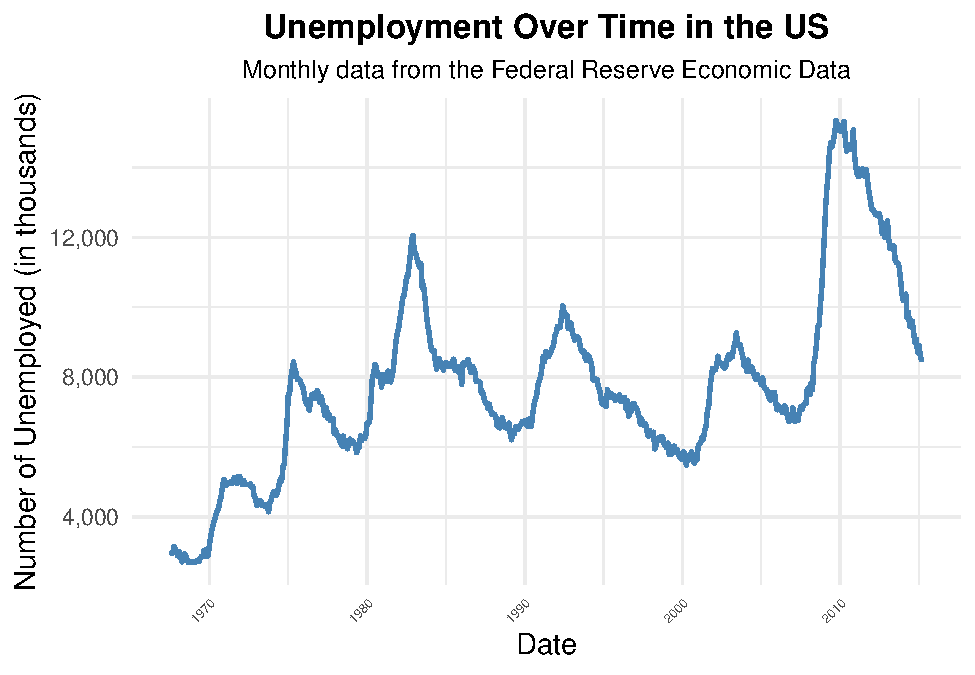
\includegraphics{P1_exercises_files/figure-latex/answer 6.1-1} \end{center}

\begin{Shaded}
\begin{Highlighting}[]
\CommentTok{\# Save the plot}
\FunctionTok{ggsave}\NormalTok{(}\AttributeTok{filename =} \StringTok{"unemployment\_plot\_improved.png"}\NormalTok{, }\AttributeTok{plot =}\NormalTok{ p, }\AttributeTok{width =} \DecValTok{8}\NormalTok{, }\AttributeTok{height =} \DecValTok{5}\NormalTok{)}
\end{Highlighting}
\end{Shaded}

\subparagraph{  Answer:}\label{answer-10}

 

\end{document}
